\documentclass[border=5pt]{standalone}
\usepackage{tikz}
\usetikzlibrary{calc}
\usepackage{amsmath}
\begin{document}
    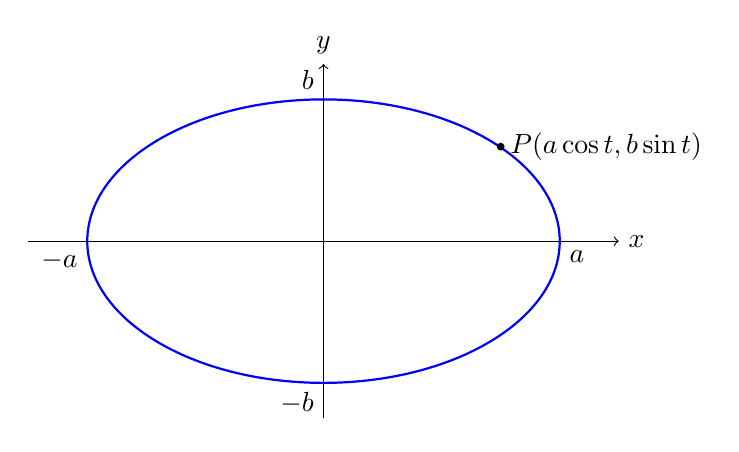
\begin{tikzpicture}[scale=1.5]
        % Draw the ellipse
        \draw[blue, thick] (0,0) ellipse (2cm and 1.2cm);

        % Draw a point P and lines to foci
        \node[circle, fill, inner sep=1pt] (P) at (1.5,0.8) {};
        \node[right] at (P) {$P(a\cos t,b\sin t)$};

        \node[below right] at (2,0) {$a$};
        \node[below left] at (-2,0) {$-a$};
        \node[above left] at (0,1.2) {$b$};
        \node[below left] at (0,-1.2) {$-b$};
        % Draw axes
        \draw[->] (-2.5,0) -- (2.5,0) node[right] {$x$};
        \draw[->] (0,-1.5) -- (0,1.5) node[above] {$y$};
    \end{tikzpicture}
\end{document}
